% Copyright 2020  Ed Bueler

\documentclass[10pt,hyperref]{beamer}

\mode<presentation>{
  \usetheme{Madrid}
  \usecolortheme{beaver}
  \setbeamercovered{transparent}  
  \setbeamerfont{frametitle}{size=\large}
}

\setbeamercolor*{block title}{bg=red!10}
\setbeamercolor*{block body}{bg=red!5}

\usepackage[english]{babel}
\usepackage[latin1]{inputenc}
\usepackage{times}
\usepackage[T1]{fontenc}
% Or whatever. Note that the encoding and the font should match. If T1
% does not look nice, try deleting the line with the fontenc.

\usepackage{empheq}
\usepackage{xspace}
\usepackage{verbatim,fancyvrb}
\usepackage{hyperref}

% If you wish to uncover everything in a step-wise fashion, uncomment
% the following command: 
%\beamerdefaultoverlayspecification{<+->}

\newcommand{\bb}{\mathbf{b}}
\newcommand{\bc}{\mathbf{c}}
\newcommand{\br}{\mathbf{r}}
\newcommand{\bx}{\mathbf{x}}
\newcommand{\by}{\mathbf{y}}
\newcommand{\bv}{\mathbf{v}}
\newcommand{\bu}{\mathbf{u}}
\newcommand{\bw}{\mathbf{w}}

\newcommand{\grad}{\nabla}

\newcommand{\CC}{\mathbb{C}}
\newcommand{\RR}{\mathbb{R}}

\newcommand{\ddt}[1]{\ensuremath{\frac{\partial #1}{\partial t}}}
\newcommand{\ddx}[1]{\ensuremath{\frac{\partial #1}{\partial x}}}
\newcommand{\Matlab}{\textsc{Matlab}\xspace}
\newcommand{\Octave}{\textsc{Octave}\xspace}
\newcommand{\MO}{\Matlab}
\newcommand{\eps}{\epsilon}

\newcommand{\ip}[2]{\left<#1,#2\right>}

\newcommand{\trefcolumn}[1]{\begin{bmatrix} \phantom{x} \\ #1 \\ \phantom{x} \end{bmatrix}}
\newcommand{\trefmatrixtwo}[2]{\left[\begin{array}{c|c|c} & & \\ #1 & \dots & #2 \\ & & \end{array}\right]}
\newcommand{\trefmatrixthree}[3]{\left[\begin{array}{c|c|c|c} & & & \\ #1 & #2 & \dots & #3 \\ & & & \end{array}\right]}
\newcommand{\trefmatrixgroups}[4]{\left[\begin{array}{c|c|c|c|c|c} & & & & & \\ #1 & \dots & #2 & #3 & \dots & #4 \\ & & & & & \end{array}\right]}

\newcommand{\blocktwo}[4]{\left[\begin{array}{c|c} #1 & #2 \\ \hline #3 & #4 \end{array}\right]}

\newcommand{\bqed}{{\color{blue}\qed}}

\newcommand{\exer}[2]{\medskip\noindent \textbf{#1.}\quad #2}


\AtBeginSection[]
{
  \begin{frame}<beamer>
    \frametitle{Outline}
    \tableofcontents[currentsection,hideallsubsections]
  \end{frame}
}

\title[Finite-dimensional spectral theory I]{Finite-dimensional spectral theory}

\subtitle{part I: from $\CC^n$ to the Schur decomposition}

\author{Ed Bueler}

\institute[MATH 617]{MATH 617 Functional Analysis}

\date{Spring 2020}

\begin{document}
\beamertemplatenavigationsymbolsempty

\begin{frame}
  \maketitle
\end{frame}


\begin{frame}{linear algebra versus functional analysis}

\begin{itemize}
\item these slides are about linear algebra, i.e.~vector spaces of finite dimension, and linear operators on those spaces, i.e.~matrices
\item one definition of \emph{functional analysis} might be: ``rigorous extension of linear algebra to $\infty$-dimensional topological vector spaces''
    \begin{itemize}
    \item[$\circ$] it is important to understand the finite-dimensional case!
    \end{itemize}
\item the goal of these part I slides is to prove the Schur decomposition and the spectral theorem for matrices
\item good references for these slides:
    \begin{itemize}
    \item[$\circ$] L.~Trefethen \& D.~Bau, \emph{Numerical Linear Algebra}, SIAM Press 1997
    \item[$\circ$] G.~Strang, \emph{Introduction to Linear Algebra}, 5th ed., Wellesley-Cambridge Press, 2016
    \item[$\circ$] G.~Golub \& C.~van Loan, \emph{Matrix Computations}, 4th ed., Johns Hopkins University Press 2013
    \end{itemize}

\end{itemize}
\end{frame}


\begin{frame}[fragile]
\frametitle{the spectrum of a matrix}

\begin{itemize}
\item the \emph{spectrum} $\sigma(A)$ of a square matrix $A$ is its set of eigenvalues
    \begin{itemize}
    \item[$\circ$] reminder later about the definition of eigenvalues
    \item[$\circ$] $\sigma(A)$ is a subset of the complex plane $\CC$
    \item[$\circ$] the plural of spectrum is \emph{spectra}; the adjectival is \emph{spectral}
    \end{itemize}
\item graphing $\sigma(A)$ gives the matrix a personality
    \begin{itemize}
    \item[$\circ$] example below: random, nonsymmetric, real $20\times 20$ matrix
    \end{itemize}
\end{itemize}

\bigskip
\begin{columns}
\begin{column}{0.5\textwidth}
\begin{Verbatim}[fontsize=\scriptsize]
>> A = randn(20,20);
>> lam = eig(A);
>> plot(real(lam),imag(lam),'o')
>> grid on
>> xlabel('Re(\lambda)')
>> ylabel('Im(\lambda)')
\end{Verbatim}
\end{column}
\begin{column}{0.5\textwidth}
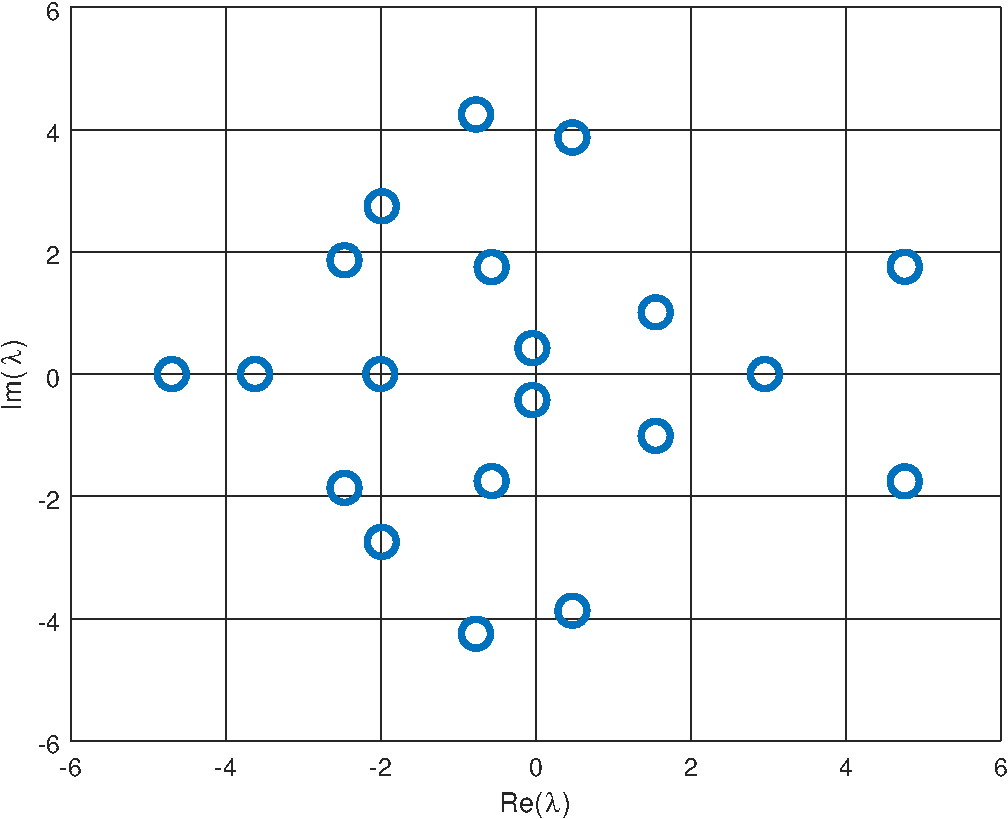
\includegraphics[width=0.9\textwidth]{figs/randspectrum}
\end{column}
\end{columns}
\end{frame}


\begin{frame}{$\CC^n$ is an inner product space}

\begin{itemize}
\item we use complex numbers $\CC$ from now on
    \begin{itemize}
    \item[$\circ$] why? because eigenvalues can be complex even for a real matrix
    \item[$\circ$] recall: if $\alpha=x+iy \in \CC$ then $\overline{\alpha} = x-iy$ is the \emph{conjugate}
    \end{itemize}
\item let $\CC^n$ be the space of (column) vectors with complex entries:
\footnotesize
    $$v = \begin{bmatrix}
    v_1 \\ \vdots \\ v_n
    \end{bmatrix}$$
\normalsize
\vspace{-2mm}
\item \textbf{definition.} an \emph{inner product} on $\CC^n$ is a function
    $$\ip{\cdot}{\cdot}:\CC^n\times \CC^n \to \CC,$$
almost-bilinear (\emph{sesquilinear}\footnote{\tiny kind of a joke, as it means ``$1\frac{1}{2}$ linear''}), with symmetry and positivity properties
\item namely, for all $u,v,w \in \CC^n$ and $\alpha\in \CC$,
    \begin{itemize}
    \item[$\circ$] $\ip{w}{u+v} = \ip{w}{u} + \ip{w}{v}$
    \item[$\circ$] $\ip{u}{\alpha v} = \alpha \ip{u}{v}$
    \item[$\circ$] $\ip{u}{v} = \overline{\ip{v}{u}}$
    \item[$\circ$] $\ip{u}{u} \ge 0$, and $\ip{u}{u}=0$ if and only if $u=0$
    \end{itemize}
\end{itemize}
\end{frame}


\begin{frame}{norm and adjoint vector}

\begin{itemize}
\item the inner product is \emph{conjugate-linear} in its first position:
    \begin{itemize}
    \item[$\circ$] $\ip{u+v}{w} = \overline{\ip{w}{u+v}} = \overline{\ip{w}{u}} + \overline{\ip{w}{v}} = \ip{u}{w} + \ip{v}{w}$
    \item[$\circ$] $\ip{\alpha u}{v} =\overline{\ip{v}{\alpha u}} = \overline{\alpha} \overline{\ip{v}{u}} =\overline{\alpha} \ip{u}{v}$
    \end{itemize}
\item \textbf{definition.}  an inner product $\ip{\cdot}{\cdot}$ induces a \emph{norm} $\|\cdot\|:\CC^n \to \RR$:
    $$\|u\| = \sqrt{\ip{u}{u}}$$
\item the \emph{hermitian transpose (adjoint)} of a vector $v\in\CC^n$ is the row vector
    $$v^* = [\overline{v_1},\dots,\overline{v_n}]$$
\item the usual inner product is just a matrix product on $\CC^n$:
\begin{align*}
\ip{u}{v} &= u^* v = \begin{bmatrix}
    \overline{u_1} & \cdots & \overline{u_n}
    \end{bmatrix} \begin{bmatrix}
    v_1 \\ \vdots \\ v_n
    \end{bmatrix}
\end{align*}
\end{itemize}
\end{frame}


\begin{frame}{linear-dependence, span, basis}

\begin{itemize}
\item \textbf{definition.}  a (finite) set of vectors $\{v_i\}_{i=1}^m \subset \CC^n$ is \emph{linearly-dependent} if there exist scalars $\alpha_i \in \CC$, not all zero, so that $\alpha_1 v_1 + \dots + \alpha_m v_m = 0$
    \begin{itemize}
    \item[$\circ$] a set of vectors is \emph{linearly-independent} if it is not linearly-dependent
    \item[$\circ$] vectors in a linearly-independent set are nonzero
    \end{itemize}
\item \textbf{definition.}  a finite set of vectors $\{v_i\}_{i=1}^m$ \emph{span} $\CC^n$ if for any $w\in \CC^n$ there exist scalars $\alpha_i$ so that $w = \alpha_1 v_1 + \dots + \alpha_m v_m$
\item \textbf{lemma.}\footnote{\url{https://en.wikipedia.org/wiki/Steinitz_exchange_lemma}}
    \begin{itemize}
    \item[$\circ$] if $\{v_i\}_{i=1}^m\subset \CC^n$ is linearly-independent then $m \le n$
    \item[$\circ$] if $\{v_i\}_{i=1}^m\subset \CC^n$ spans $\CC^n$ then $m \ge n$
    \end{itemize}
\item \textbf{definition.} a finite set of vectors $\{v_i\}_{i=1}^m \subset \CC^n$ is a \emph{basis} if the set is linearly-independent and it spans $\CC^n$
    \begin{itemize}
    \item[$\circ$] by the lemma, $m=n$
    \item[$\circ$] the \emph{dimension} $n$ is well-defined as the number of elements in a basis
    \end{itemize}
\end{itemize}
\end{frame}


\begin{frame}{linear operators and matrices}

\begin{itemize}
\item \textbf{definition.}  $A:\CC^n \to \CC^n$ is \emph{linear} if $A(\alpha u+\beta v) = \alpha A(u) + \beta A(v)$
    \begin{itemize}
    \item[$\circ$] we call such a function a \emph{linear operator} and we write $Au=A(u)$
    \end{itemize}
\item given a basis, one may represent a linear operator as a (square) \emph{matrix}
    \begin{itemize}
    \item[$\circ$] matrix multiplication is just function composition
    \end{itemize}
\item \textbf{definition.} $A$ is \emph{invertible} if there exists $B$ so that $AB=BA=I$
\item \textbf{lemma.} matrix $A$ is invertible if and only if its columns form a basis
\end{itemize}
\end{frame}


\begin{frame}{meanings of matrix multiplication}

\begin{itemize}
\item the ``purpose'' of a matrix $A \in \CC^{n\times m}$ is to multiply vectors $u\in \CC^m$
    \begin{itemize}
    \item[$\circ$] a matrix is merely the representation of a linear operator
    \item[$\circ$] operations on entries, e.g.~$\det()$ or row operations, are less fundamental
    \end{itemize}
\item when you see ``$Au$'' remember two views:
\small
\begin{align*}
A u &= \left[\begin{array}{ccc}
& r_1 & \\ \hline
& r_2 & \\ \hline
& \vdots & \\ \hline
& r_n &
\end{array}\right] u = \begin{bmatrix} r_1 u \\ r_2 u \\ \vdots \\ r_n u \end{bmatrix}  \\
A u &= \trefmatrixthree{a_1}{a_2}{a_m} \begin{bmatrix} u_1 \\ u_2 \\ \vdots \\ u_m \end{bmatrix} = u_1 \trefcolumn{a_1} + u_2 \trefcolumn{a_2} + \dots + u_m \trefcolumn{a_m}
\end{align*}
\normalsize
    \begin{itemize}
    \item[$\circ$] $A$ acts on $u$ acts from the left; each entry is an inner product
    \item[$\circ$] $u$ acts from the right on $A$; get a linear-combination of columns
    \end{itemize}
\item also: if $A \in \CC^{n\times n}$ is invertible then $A^{-1}w$ computes the coefficients of $w$ in the basis of columns of $A$
\end{itemize}
\end{frame}


\begin{frame}{adjoints, orthonormal bases, and unitary matrices}

\begin{itemize}
\item \textbf{definition.} the \emph{hermitian transpose} or \emph{adjoint} of $A\in \CC^{n\times m}$ is $A^* \in \CC^{m\times n}$:
    $$A = \begin{bmatrix}
    a_{11} & a_{12} & \dots & a_{1m} \\
    a_{21} & a_{22} &       & a_{2m} \\
    \vdots &        & \ddots& \vdots \\
    a_{n1} & a_{n2} & \dots & a_{nm} \end{bmatrix}
    \quad \to \quad
    A^* = \begin{bmatrix}
    \overline{a_{11}} & \overline{a_{21}} & \dots & \overline{a_{n1}} \\
    \overline{a_{12}} & \overline{a_{22}} &       & \overline{a_{n2}} \\
    \vdots            &                   & \ddots& \vdots \\
    \overline{a_{1m}} & \overline{a_{2m}} & \dots & \overline{a_{nm}} \end{bmatrix}$$
\item \textbf{definition.} a basis $\{v_i\}_{i=1}^n$ of $\CC^n$ is \emph{orthonormal} (ON) if
\small
    $$\ip{v_i}{v_j} =v_i^* v_j = \delta_{ij} = \begin{cases} 1, & i=j \\ 0, & i\ne j \end{cases}$$
\normalsize
\vspace{-2mm}
    \begin{itemize}
    \item[$\circ$] ``ortho'' means $\ip{v_i}{v_j}=0$ if $i\ne j$ and ``normal'' means $\|v_i\|=1$
    \end{itemize}
\item \textbf{definition.} a matrix $U$ is \emph{unitary} if $U^* U = I$, thus $U^{-1}=U^*$
\item \textbf{lemma.} a matrix $U$ is unitary if and only if its columns form an ON basis
    \begin{itemize}
    \item[\emph{proof.}] The entries of a matrix product are inner products between the rows of the left factor and the columns of the right factor.  The entries of $I$ are $\delta_{ij}$. \bqed
    \end{itemize}
\end{itemize}
\end{frame}


\begin{frame}{Gram-Schmidt process}

\label{GSformulas}
\begin{itemize}
\item given a set of vectors $\{w_i\}_{i=1}^m \subset \CC^n$ we can generate new orthonormal vectors which span the same subspace
    \begin{itemize}
    \item[$\circ$] if the original set spans $\CC^n$ then the result is an ON basis
    \end{itemize}
\item formulas:
\begin{align*}
\tilde v &= w_1 \quad \to & v_1 &= \tilde v/\|\tilde v\| \\
\tilde v &= w_2 - \ip{v_1}{w_2} v_1 \quad \to & v_2 &= \tilde v/\|\tilde v\| \\
\tilde v &= w_3 - \ip{v_1}{w_3} v_1 - \ip{v_2}{w_3} v_2 \quad \to & v_3 &= \tilde v/\|\tilde v\| \\
\tilde v &= w_4 - \ip{v_1}{w_4} v_1 - \ip{v_2}{w_4} v_2 - \ip{v_3}{w_4} v_3 \quad \to & v_4 &= \tilde v/\|\tilde v\| \\
&\vdots & &\vdots
\end{align*}
\vspace{-4mm}
    \begin{itemize}
    \item[$\circ$] exception: if $\tilde v=0$ at any stage then we ignore that $w_i$ and skip to $w_{i+1}$
    \item[$\circ$] notice the triangular structure
    \end{itemize}
\item \textbf{lemma.}
    \begin{itemize}
    \item[$\circ$] $\{v_i\}$ is ON
    \item[$\circ$] $\operatorname{span}\{v_i\} = \operatorname{span}\{w_i\}$
    \item[$\circ$] if $\{w_i\}_{i=1}^m$ spans $\CC^n$, thus $m\ge n$, then $\{v_i\}_{i=1}^n$ is an ON basis
    \end{itemize}
\end{itemize}
\end{frame}


\begin{frame}{Gram-Schmidt \underline{is} QR}

\begin{itemize}
\item the Gram-Schmidt formulas are of the form
\small
    $$\alpha_i v_i \stackrel{\ast}{=} w_i - \sum_{j=1}^{i-1} \beta_{ji} v_j$$
\normalsize
where $\alpha_i=\|\tilde v\|$ is a normalization constant and $\beta_{ji}=\ip{v_j}{w_i}$
\item moving the $v_i$ to the left in $\ast$, and writing vectors as columns gives
\small
    $$\trefmatrixthree{v_1}{v_2}{v_m}
      \begin{bmatrix} \alpha_1 & \beta_{12} & \beta_{13} & \dots & \beta_{1m} \\
                      0        & \alpha_2   & \beta_{23} &       & \beta_{2m} \\
                      \vdots   &            &            & \ddots & \vdots \\
                      0        & 0          & \dots      &       & \alpha_m \end{bmatrix}
      = \trefmatrixthree{w_1}{w_2}{w_m}$$
\normalsize
\item this is a ``reduced'' QR decomposition
    $$\hat Q \hat R = A$$

\vspace{-1mm}
    \begin{itemize}
    \item[$\circ$] $A$ is $n\times m$ and contains the original vectors $w_i$,
    \item[$\circ$] $\hat Q$ is the same size as $A$ and contains the ON vectors $v_i$,
    \item[$\circ$] and  $\hat R$ is (upper-) right-triangular and $m\times m$, thus small if $m\ll n$
    \end{itemize}
\item if $m=n$ and columns of $A$ span $\CC^n$ ($A$ has \emph{full rank}) then $Q$ is unitary

\medskip
\footnotesize
\item methods: numerical QR uses Householder, not Gram-Schmidt, for stability reasons
\end{itemize}
\end{frame}


\begin{frame}[fragile]
\frametitle{Gram-Schmidt process: example 1}

\begin{itemize}
\item suppose we have $m=3$ vectors in $\CC^3$:
\small
    $$w_1 = \begin{bmatrix} 9 \\ 3 \\ 4 \end{bmatrix}, \quad w_2 = \begin{bmatrix} 1 \\ 6 \\ 9 \end{bmatrix}, \quad w_3 = \begin{bmatrix} 6 \\ 7 \\ 3 \end{bmatrix}$$
\normalsize
\item applying the formulas on slide \pageref{GSformulas}:
\small
    $$v_1 = \begin{bmatrix} 0.87416 \\ 0.29139 \\ 0.38851 \end{bmatrix}, \quad v_2 = \begin{bmatrix} -0.48456 \\ 0.46984 \\ 0.73787 \end{bmatrix}, \quad v_3 = \begin{bmatrix} -0.03247 \\ 0.83327 \\ -0.55191 \end{bmatrix}$$
\normalsize
\item compare this \Matlab calculation:
\begin{Verbatim}[fontsize=\scriptsize]
>> A = [9 1 6; 3 6 7; 4 9 3];
>> [Q,R] = qr(A)
Q =
    -0.87416     0.48456    0.032465
    -0.29139    -0.46984    -0.83327
    -0.38851    -0.73787     0.55191
R =
     -10.296     -6.1191     -8.4502
           0     -8.9753     -2.5952
           0           0     -3.9824
\end{Verbatim}
\end{itemize}
\end{frame}


\begin{frame}[fragile]
\frametitle{Gram-Schmidt process: example 2}

\begin{itemize}
\item what is this \Matlab calculation doing?:

\medskip
\begin{Verbatim}[fontsize=\scriptsize]
>> x = (-1:.01:1)';
>> A = [x.^0 x.^1 x.^2 x.^3 x.^4];
>> size(A)
ans =
      201        5
>> [Q,R] = qr(A,0);
>> size(Q)
ans =
      201        5
>> plot(x,Q),  xlabel x
>> axis tight,  grid on
\end{Verbatim}

\vspace{-18mm}
\hfill 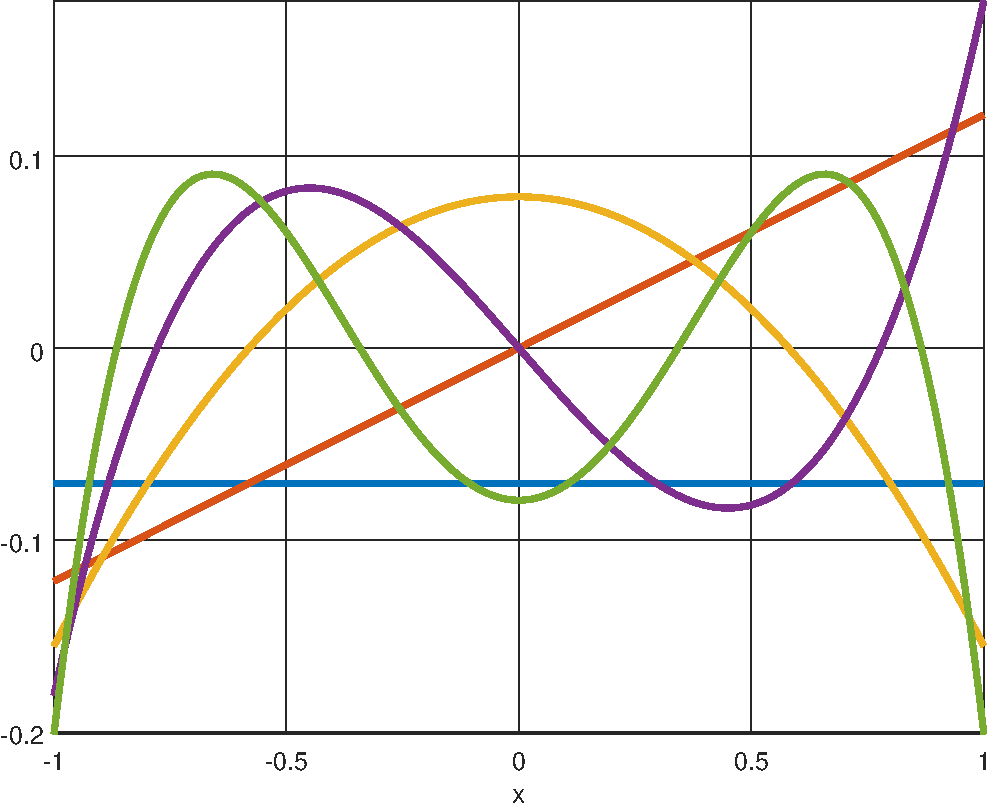
\includegraphics[width=0.55\textwidth]{figs/legendre} \quad 

\item the plot shows Legendre polynomials up to degree 4
\end{itemize}
\end{frame}


\begin{frame}{technique: extend to an ON basis}

\begin{itemize}
\item a key technique, for proofs related to spectral theory, is to extend $m<n$ ON vectors to an ON basis
\item let $\{e_i\}_{i=1}^n$ be the standard basis of $\CC^n$, with $(e_i)_j = \delta_{ij}$
\item \textbf{method.} given ON vectors $\{u_1,\dots,u_m\}$, for $1 \le m<n$, apply the Gram-Schmidt process to
    $$w_1=u_1, \quad \dots \quad w_m=u_m, \quad w_{m+1}=e_1, \quad \dots \quad w_{m+n}=e_n$$

\vspace{-2mm}
    \begin{itemize}
    \item[$\circ$] note: this set of $m+n$ vectors does indeed span $\CC^n$!
    \item[$\circ$] the first $m$ steps of G.-S. are trivial, but after that there will be discarded vectors because $\|\tilde v\|=0$
    \item[$\circ$] result is ON set $\{v_i\}_{i=1}^n$ where first $m$ vectors were given
    \end{itemize}
\item as matrices, if $\hat Q$ has ON columns then we extend to a unitary matrix:
\small
    $$\hat Q = \trefmatrixtwo{u_1}{u_m} \quad \to \quad Q = \trefmatrixgroups{u_1}{u_m}{v_{m+1}}{v_n}$$
\end{itemize}
\end{frame}


\begin{frame}{eigenvalues and eigenvectors}

\begin{itemize}
\item \textbf{definition.}  given a square matrix $A \in \CC^{n\times n}$, $v\in\CC^n$ is an \emph{eigenvector} if $v\ne 0$ and if there exists $\lambda\in \CC$ so that
    $$A v = \lambda v$$

\vspace{-2mm}
    \begin{itemize}
    \item[$\circ$] $\lambda$ is the \emph{eigenvalue} for $v$
    \item[$\circ$] idea: $A$ acts in a simple way on (multiples of) $v$, simply by scaling
    \end{itemize}
\item \textbf{definition.}  the \emph{spectrum} $\sigma(A)$ of $A \in \CC^{n\times n}$ is the set of its eigenvalues
\item \textbf{lemma.} $\lambda\in\sigma(A)$ if and only if $\det(\lambda I - A)=0$
    \begin{itemize}
    \item[\emph{proof.}] $\lambda\in\sigma(A) \, \iff \, \exists \text{ nonzero soln.~to } (\lambda I - A) v = 0 \, \iff \, \det(\lambda I - A)=0$ \bqed
    \end{itemize}
\item \textbf{corollary.} $\sigma(A)$ is nonempty 
    \begin{itemize}
    \item[\emph{proof.}] $p(\lambda) = \det(\lambda I - A)$ is a degree $n$ polynomial, which has a root $\lambda\in\CC$ \bqed
    \end{itemize}
\end{itemize}
\end{frame}


\begin{frame}{hermitian matrices and their eigenvalues}

\begin{itemize}
\item general facts about adjoints:
    \begin{itemize}
    \item[$\circ$] $(AB)^*=B^*A^*$
    \item[$\circ$] in usual inner product $\ip{v}{w}=v^*w$: \, $\ip{v}{Aw} = \ip{A^* v}{w}$
    \end{itemize}
\item \textbf{definition.} $A \in \CC^{n\times n}$ is \emph{hermitian} if $A^*=A$
    \begin{itemize}
    \item[$\circ$] also called \emph{self-adjoint}
    \item[$\circ$] $\overline{a_{ij}} = a_{ji}$ \dots so the diagonal entries of $A$ are real
    \item[$\circ$] in usual inner product $\ip{v}{w}=v^*w$: \, $\ip{v}{Aw} = \ip{A v}{w}$
    \item[$\circ$] if $A$ has real entries then $A^\top=A$, and $A$ is \emph{symmetric}
    \end{itemize}
\item \textbf{lemma.} if $A$ is hermitian and $\lambda \in \sigma(A)$ then $\lambda$ is real
    \begin{itemize}
    \item[\emph{proof.}] a classic exercise \dots for you
    \end{itemize}
\item \textbf{lemma.} if $A$ is hermitian and $v,w \in \CC^n$ are eigenvectors associated to distinct eigenvalues then $v,w$ are orthogonal
    \begin{itemize}
    \item[\emph{proof.}] a classic exercise: if $Av=\lambda v$ and $Aw=\mu w$ then $\lambda,\mu$ are real so
    $$(\lambda-\mu) \ip{v}{w} = \ip{\lambda v}{w} - \ip{v}{\mu w} = \ip{Av}{w} - \ip{v}{Aw} = \ip{v}{Aw} - \ip{v}{Aw} = 0,$$
and we have assumed $\lambda-\mu \ne 0$ \bqed
    \end{itemize}
\end{itemize}
\end{frame}


\begin{frame}{eigendecompositions}

\begin{itemize}
\item for any $A\in\CC^{n\times n}$, if $v_1,\dots,v_m$ are eigenvectors with eigenvalues $\lambda_1,\dots,\lambda_m$ then we can collect the statements $A v_i=\lambda_i v_i$ as
\small
    $$A \trefmatrixtwo{v_1}{v_m} =  \trefmatrixtwo{v_1}{v_m} \begin{bmatrix} \lambda_1 & & \\ & \ddots & \\ & & \lambda_m \end{bmatrix}$$
\normalsize
\item equivalently:
    $$A V = V \Lambda$$
\item if $V$ is square and invertible then we have a decomposition of $A$:
    $$A = V \Lambda V^{-1}$$
\item why does this matter?  often $A$ is iterated, or a polynomial is applied,
    $$A^k = (V \Lambda V^{-1})^k = V \Lambda V^{-1}V \Lambda V^{-1}\dots V \Lambda V^{-1} = V \Lambda^k V^{-1}$$
    $$p(A) = V\, p(\Lambda) V^{-1}$$

    \begin{itemize}
    \item[$\circ$] $\Lambda^k$, $p(\Lambda)$ are easy-to-understand diagonal matrices
    \end{itemize}
\end{itemize}
\end{frame}


\begin{frame}{similarity and diagonalizability}

\begin{itemize}
\item \textbf{definition.} $A,B$ are \emph{similar} if there exists $V$ invertible so that
    $$A = V B V^{-1}$$
\item \textbf{lemma.} if $A,B$ are similar then $\sigma(A)=\sigma(B)$
    \begin{itemize}
    \item[\emph{proof.}] noting $\det(TS)=\det(T)\det(S)$, we have
\begin{align*}
\det(\lambda I - A) &= \det(\lambda VV^{-1} - V B V^{-1}) = \det(V) \det(\lambda I - B) \det(V^{-1}) \\
    &= \det(V) \det(\lambda I - B) \det(V)^{-1} = \det(\lambda I - B) \bqed
\end{align*}
    \end{itemize}
\item \textbf{lemma.} if $A$ is triangular or diagonal then $\sigma(A)=\{a_{ii}\}$  (diagonal entries)
    \begin{itemize}
    \item[\emph{proof.}] $\det(\lambda I - A) = \prod_{i=1}^n \lambda-a_{ii}$ \bqed
    \end{itemize}
\item \textbf{definition.} $A$ is \emph{diagonalizable} if there exists $V$ invertible and $\Lambda$ diagonal so that
    $$A = V \Lambda V^{-1}$$

    \begin{itemize}
    \item[$\circ$] equivalently, $A$ is diagonalizable if it is similar to a diagonal matrix
    \item[$\circ$] not every square matrix is diagonalizable!
    \end{itemize}
\end{itemize}
\end{frame}


\begin{frame}{non-diagonalizable (``defective'') matrices}

\begin{itemize}
\item if you pick a matrix $A\in\CC^{n\times n}$ at random then it will be diagonalizable with probability one,\footnote{\tiny this assumes only that your probability measure has a continuous density with respect to Lebesgue measure} but non-diagonalizable matrices exist
\item simplest example (\emph{check all this!}): \quad $A = \begin{bmatrix} 0 & 1 \\ 0 & 0 \end{bmatrix}$
    \begin{itemize}
    \item[$\circ$] note $A$ is triangular, and $\sigma(A) = \{0\}$
    \item[$\circ$] if $A=V\Lambda V^{-1}$ for $V$ invertible then columns of $V$ would be linearly-independent eigenvectors: $Av_1=0v_1$ and $Av_2=0v_2$
    \item[$\circ$] but in fact $(\lambda I - A) v = 0$ has only a one-dimensional solution space
    \end{itemize}
\item all non-diagonal examples $A$ are built by choosing $J$ to be a ``non-diagonal Jordan form,'' with at least one block of this form on the diagonal:
\footnotesize
    $$\begin{bmatrix} \lambda & 1 \\ 0 & \lambda \end{bmatrix}, \quad \begin{bmatrix} \lambda & 1 & 0 \\ 0 & \lambda & 1 \\ 0 & 0 & \lambda \end{bmatrix}, \quad \begin{bmatrix} \lambda & 1 & 0 & 0 \\ 0 & \lambda & 1 & 0 \\ 0 & 0 & \lambda & 1 \\ 0 & 0 & 0 & \lambda \end{bmatrix}, \quad \dots,$$
\normalsize
and with $J$ otherwise diagonal, and defining $A=VJV^{-1}$ for some invertible $V$
\end{itemize}
\end{frame}


\begin{frame}{eigenvalue-revealing decompositions}

\begin{itemize}  
\item there are four famous ``eigenvalue-revealing'' decompositions of square matrices $A\in\CC^{n\times n}$:
\begin{align*}
A &= V \Lambda V^{-1} & &\text{if $A$ is diagonalizable} \\
A &= V J V^{-1} & &\text{\underline{for any $A$}, where $J$ is special triangular \emph{Jordan form}} \\
A &= Q \Lambda Q^* & &\text{if $A$ is hermitian, where $Q$ is unitary} \\
A &= Q T Q^* & &\text{\underline{for any $A$}, where $T$ is triangular and $Q$ is unitary}
\end{align*}
\item respectively: \hfill \small \Matlab commands\normalsize
    \begin{itemize}
    \item[] $A = V \Lambda V^{-1}$ is \emph{eigendecomposition} or \emph{diagonalization} \hfill \texttt{eig(A)}
    \item[] $A = V J V^{-1}$ is \emph{Jordan canonical form}
    \item[] $A = Q \Lambda Q^*$ is \emph{spectral theorem} \hfill \texttt{eig(A)}
    \item[] $A = Q T Q^*$ is \emph{Schur decomposition} \hfill \texttt{schur(A,'complex')}
    \end{itemize}

\medskip
\item the Jordan canonical form cannot be computed if rounding errors exist\footnote{\tiny G.~Golub \& J.~Wilkinson 1976, \emph{Ill-conditioned eigensystems and the computation of the Jordan canonical form}, SIAM Review 18(4), 578--619}
\item the Schur decomposition is the most important in practice, as it always exists and it can be stably computed over $\RR$ or $\CC$
\end{itemize}
\end{frame}


\begin{frame}{Schur decomposition}

\begin{itemize}
\item \textbf{theorem.} if $A\in \CC^{n\times n}$ then there exist $T,Q\in \CC^{n\times n}$, with $T$ upper-triangular and $Q$ unitary, so that
    $$A = Q T Q^*$$

\vspace{-2mm}
    \begin{itemize}
    \footnotesize
    \item[\emph{proof.}] Induct on $n$.  If $n=1$ then the result follows with $T=A=[a_{11}]$ and $Q=I=[1]$.

\quad For $n>1$ let $v\ne 0$ be an eigenvector of $A$, with eigenvalue $\lambda$. Let $u_1=v/\|v\|$ and extend to a unitary matrix:
    $$U = \trefmatrixthree{u_1}{u_2}{u_n}$$
Apply $A$ and note that $Au_1=\lambda u_1$:
    $$AU = \trefmatrixthree{\lambda_1 u_1}{A u_2}{A u_n}$$
Apply $U^*=U^{-1}$, observe that $U^*Au_1 = \lambda_1 U^* u_1 = \lambda_1 e_1$, and write $w_j=U^*Au_j$:
    $$U^*AU = \trefmatrixthree{\lambda_1 e_1}{w_2}{w_n}$$
(We don't care about the form of the vectors $w_2,\dots,w_n \in \CC^n$.)
    \end{itemize}
\normalsize
\end{itemize}
\end{frame}


\begin{frame}{Schur decomposition, proof cont.}

\begin{itemize}
\item[]
    \begin{itemize}
    \footnotesize
    \item[] \quad We have made progress toward upper-triangular form.  In fact, we may write
    $$U^*AU = \blocktwo{\lambda_1}{z^*}{0}{M}$$
for some $z\in \CC^{n-1}$ and $M\in \CC^{n-1 \times n-1}$.  By induction, $M$ has a Schur decomposition, $M=\hat Q \hat T \hat Q^*$, where $\hat T,\hat Q$ are the same size as $M$.  Note that
    $$\blocktwo{1}{0}{0}{\hat Q}$$
is unitary.  Now we can transform the whole matrix $U^*AU$ to triangular form:
    $$\blocktwo{1}{0}{0}{\hat Q^*} U^*AU \blocktwo{1}{0}{0}{\hat Q} = \blocktwo{\lambda_1}{z^*\hat Q}{0}{\hat T}$$
Now let
    $$T = \blocktwo{\lambda_1}{z^*\hat Q}{0}{\hat T}, \quad Q = U \blocktwo{1}{0}{0}{\hat Q}$$
We have $A=Q^*T Q$. \bqed
    \end{itemize}
\normalsize

\bigskip
\item note key steps at start of proof: ``let $v\ne 0$ be an eigenvector of $A$'' and ``extend to a unitary matrix''
\end{itemize}
\end{frame}


\begin{frame}[fragile]
\frametitle{Schur decomposition: computed examples}

\begin{itemize}
\item note the diagonal entries of $T$ contain the eigenvalues (compare \texttt{eig(A)})
\item example 1: general case
\begin{Verbatim}[fontsize=\scriptsize]
>> A=randn(4,4);
>> [Q,T] = schur(A)
Q =
  0.25290  0.78457  -0.32111  0.46624
  0.12587  0.07899  -0.70892  -0.68945
  -0.82852  0.47758  0.15009  -0.25088
  -0.48348  -0.38746  -0.60974  0.49431
T =
  1.94208  -1.22908  -1.37600  -0.70166
  0.00000  -1.81581  0.21700  -0.51769
  0.00000  0.00000  0.69477  -1.15766
  0.00000  0.00000  0.00000  -0.59708
>> norm(A-Q*T*Q')
ans =    2.0928e-15
\end{Verbatim}
    \begin{itemize}
    \footnotesize
    \item[$\circ$] we just got lucky; see \, \texttt{help schur}\, for real vs.~complex Schur decompositions
    \end{itemize}
\item example 2: hermitian case
\begin{Verbatim}[fontsize=\scriptsize]
>> B = randn(4,4);  A = B + B';
>> [Q,T] = schur(A);  T
T =
  3.42692  -0.00000  -0.00000  -0.00000
  0.00000  0.96497  0.00000  -0.00000
  0.00000  0.00000  -2.92548  0.00000
  0.00000  0.00000  0.00000  -4.61828
\end{Verbatim}
\end{itemize}
\end{frame}


\begin{frame}{normal matrices}

\begin{itemize}
\item \textbf{lemma.} if $A$ is hermitian then the Schur decomposition is a unitary diagonalization
    \begin{itemize}
    \item[\emph{proof.}] $A^* = A$ so $Q T^* Q^* = Q T Q^*$ so $T^*=T$ \bqed
    \end{itemize}
\item there is a larger class of matrices where this happens
\item \textbf{definition.} $A\in \CC^{n\times n}$ is \emph{normal} if $AA^*=A^*A$
\item examples:
    \begin{itemize}
    \item[$\circ$] $A$ hermitian $\implies$ $A$ normal
    \item[$\circ$] $U$ unitary $\implies$ $U$ normal
    \item[$\circ$] $S$ skew-hermitian\footnote{\scriptsize $S^*=-S$} $\implies$ $S$ normal
    \end{itemize}
\end{itemize}
\end{frame}


\begin{frame}{the spectral theorem}

\begin{itemize}
\item \textbf{corollary (spectral theorem).} if $A$ is normal then there exists $\Lambda$ diagonal and $Q$ unitary so that
    $$A=Q \Lambda Q^*$$

    \begin{itemize}
    \item[\emph{proof.}] From the Schur decomposition, $A=QTQ^*$.  Since $A$ is normal, it follows that $TT^*=T^*T$.  But $T$ is upper-triangular, so
    $$T = \blocktwo{t_{11}}{z^*}{0}{R}$$
where $R$ is also upper triangular.  An easy calculation shows $(TT^*)_{11} = |t_{11}|^2 + \|z\|^2$ while $(T^*T)_{11} = |t_{11}|^2$.  Thus $z=0$.  Now induct to show $T$ is diagonal. \bqed
    \end{itemize}
\end{itemize}
\end{frame}


\begin{frame}{where we stand}

\begin{itemize}
\item in part II we will discuss consequences of the spectral theorem
\item \dots and get to the singular value decomposition
\item almost everything we do will have some kind of analog in $\infty$-dimensions
\item \dots and appear somewhere in our textbook\footnote{Muscat, \emph{Functional Analysis}; see Chapter 10 for Hilbert spaces}
\item \dots but most proof steps do not extend directly to $\infty$-dimensions
\item \textbf{questions.} in an $\infty$-dimensional Hilbert space,
    \begin{itemize}
    \item[$\circ$] what is the meaning of ``span'' and ``basis''?
    \item[$\circ$] are matrices meaningful?
    \item[$\circ$] is a one-to-one linear operator invertible?
    \item[$\circ$] does the Gram-Schmidt process work as before?
    \item[$\circ$] does every linear operator have an eigenvector?
    \item[$\circ$] is there a Schur decomposition of every linear operator?
    \item[$\circ$] is there a spectral theorem of hermitian or normal operators?
    \end{itemize}
\end{itemize}
\end{frame}

\end{document}

